\section{Claw-free cubic graphs}

In this section we study $3$-dynamic colorings of claw-free cubic graphs.
A \emph{diamond} is an induced subgraph isomorphic to $K_4 - e$. 
We say that two diamonds are \emph{adjacent} if there exists an edge joining a degree-$2$ vertex of one diamond to a degree-$2$ vertex of the other. 
Contracting each diamond to a single vertex and preserving these adjacencies yields an auxiliary graph; if this graph is a path, we call the corresponding subgraph a \emph{string of diamonds}, and if it is a cycle, we call it a \emph{ring of diamonds}.


We have the next observation, whose proof is direct by inspection
(Figure~\ref{fig:cubic-claw-free-ring-string}a).

\begin{observation}\label{obs:ringX3leq5}
    If $G$ is a ring of diamonds then $\chi_3(G) \leq 5$.
\end{observation}

\begin{figure}[H]
    \centering
    \setcounter{subfigure}{0}

    \begin{subfigure}[b]{0.48\textwidth}
        \centering
        % \tikzexternaldisable


\tikzsetnextfilename{cubic-claw-free-ring}
\begin{tikzpicture}[scale=0.5, transform shape]
\centering
    \begin{scope}[yshift=1cm]
    \node[vertex,label=below:$0$] (A0) {};
    \node[vertex,label=below:$3$] (A1) at ($(A0)+(4,0)$) {};
    \node[vertex, draw=black, thick,label=above:$1$] (A2) at ($(A0)+(2,1)$) {};
    \node[vertex,label=below:$2$] (A3) at ($(A0)+(2,-1)$) {};
    \foreach \source/\dest in {A0/A2,A0/A3,A1/A2,A1/A3,A2/A3}
        \path[black edge] (\source) -- (\dest);
    \end{scope}

    \draw[black edge] (A2) -- (A3);

    \begin{scope}[xshift=5cm,yshift=1cm,rotate=45]
    \node[vertex,label=below:$0$] (B0) {};
    \node[vertex,label=below:$3$] (B1) at ($(B0)+(4,0)$) {};
    \node[vertex,draw=black,thick,label=above:$1$] (B2) at ($(B0)+(2,1)$) {};
    \node[vertex,label=below:$2$] (B3) at ($(B0)+(2,-1)$) {};
    \foreach \source/\dest in {B0/B2,B0/B3,B1/B2,B1/B3,B2/B3}
        \path[black edge] (\source) -- (\dest);
    \end{scope}

    \draw[black edge] (B2) -- (B3);

    \begin{scope}[xshift=7.8cm,yshift=5cm,rotate=135]
    \node[vertex,label=below:$0$] (C0) {};
    \node[vertex,label=below:$3$] (C1) at ($(C0)+(4,0)$) {};
    \node[vertex,draw=black,thick,label=above:$1$] (C2) at ($(C0)+(2,1)$) {};
    \node[vertex,label=below:$2$] (C3) at ($(C0)+(2,-1)$) {};
    \foreach \source/\dest in {C0/C2,C0/C3,C1/C2,C1/C3,C2/C3}
        \path[black edge] (\source) -- (\dest);
    \end{scope}

    \draw[black edge] (C2) -- (C3);

    \begin{scope}[yshift=7.85cm]
    \node[vertex,label=below:$3$] (D0) {};
    \node[vertex,label=below:$0$] (D1) at ($(D0)+(4,0)$) {};
    \node[vertex,label=above:$2$] (D2) at ($(D0)+(2,1)$) {};
    \node[vertex,draw=black,thick,label=below:$1$] (D3) at ($(D0)+(2,-1)$) {};
    \foreach \source/\dest in {D0/D2,D0/D3,D1/D2,D1/D3,D2/D3}
        \path[black edge] (\source) -- (\dest);
    \end{scope}

    \draw[black edge] (D2) -- (D3);

    \begin{scope}[xshift=-4cm,yshift=3.85cm,rotate=-45]
    \node[vertex,label=below:$0$] (F0) {};
    \node[vertex,label=below:$3$] (F1) at ($(F0)+(4,0)$) {};
    \node[vertex,draw=black,thick,label=above:$1$] (F2) at ($(F0)+(2,1)$) {};
    \node[vertex,label=below:$2$] (F3) at ($(F0)+(2,-1)$) {};
    \foreach \source/\dest in {F0/F2,F0/F3,F1/F2,F1/F3,F2/F3}
        \path[black edge] (\source) -- (\dest);
    \end{scope}

    \draw[black edge] (F2) -- (F3);

    \begin{scope}[xshift=-4cm,yshift=5cm,rotate=45]
    \node[vertex,label=below:$3$] (E0) {};
    \node[vertex,label=below:$0$] (E1) at ($(E0)+(4,0)$) {};
    \node[vertex,label=above:$2$] (E2) at ($(E0)+(2,1)$) {};
    \node[vertex,draw=black,thick,label=below:$1$] (E3) at ($(E0)+(2,-1)$) {};
    \foreach \source/\dest in {E0/E2,E0/E3,E1/E2,E1/E3,E2/E3}
        \path[black edge] (\source) -- (\dest);
    \end{scope}

    \draw[black edge] (E2) -- (E3);

    % Aristas entre los diamantes
    \draw[black edge] (A0) -- (F1);
    \draw[black edge] (D0) -- (E1);
    \draw[black edge] (E0) -- (F0);
    \draw[black edge] (C1) -- (D1);
    \draw[black edge] (B1) -- (C0);
    \draw[black edge] (A1) -- (B0);

\end{tikzpicture}
        \caption{$ $}
        \label{fig:cubic-claw-free-ring}
    \end{subfigure}
    \hfill
    \begin{subfigure}[b]{0.48\textwidth}
        \centering
        % \tikzexternaldisable

\tikzsetnextfilename{fig-cubic-string}
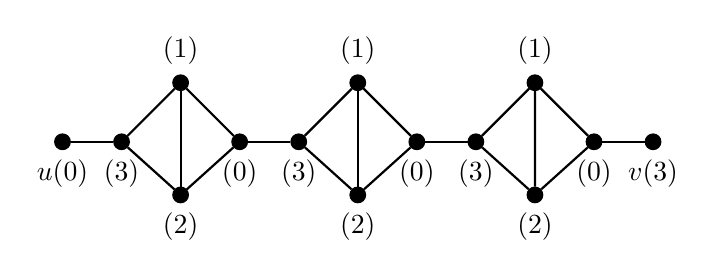
\begin{tikzpicture}[scale=0.75,
    vertex/.style={circle, draw, fill=black, inner sep=2pt},
    redvertex/.style={circle, draw, fill=red, inner sep=2pt},
    edge/.style={draw, thick}
]

% (mismo dibujo)
\node[vertex, label=below:$u (0)$] (u) at (0,0) {};
\node[vertex,label=below:$(3)$] (a1) at (1,0) {};
\draw[edge] (u) -- (a1);

\node[vertex, label=above:$(1)$] (t1) at (2,1) {};
\node[vertex,label=below:$(2)$] (b1) at (2,-0.9) {};
\node[vertex,label=below:$(0)$] (c1) at (3,0) {};
\draw[edge] (a1) -- (t1);
\draw[edge] (a1) -- (b1);
\draw[edge] (b1) -- (c1);
\draw[edge] (c1) -- (t1);
\draw[edge] (t1) -- (b1);

\node[vertex,label=below:$(3)$] (a2) at (4,0) {};
\draw[edge] (c1) -- (a2);

\node[vertex, label=above:$(1)$] (t2) at (5,1) {};
\node[vertex,label=below:$(2)$] (b2) at (5,-0.9) {};
\node[vertex,label=below:$(0)$] (c2) at (6,0) {};
\draw[edge] (a2) -- (t2);
\draw[edge] (a2) -- (b2);
\draw[edge] (b2) -- (c2);
\draw[edge] (c2) -- (t2);
\draw[edge] (t2) -- (b2);

\node[vertex,label=below:$(3)$] (a3) at (7,0) {};
\draw[edge] (c2) -- (a3);

\node[vertex, label=above:$(1)$] (t3) at (8,1) {};
\node[vertex, label=below:$(2)$] (b3) at (8,-0.9) {};
\node[vertex, label=below:$(0)$] (c3) at (9,0) {};
\draw[edge] (a3) -- (t3);
\draw[edge] (a3) -- (b3);
\draw[edge] (b3) -- (c3);
\draw[edge] (c3) -- (t3);
\draw[edge] (t3) -- (b3);

\node[vertex, label=below:$v (3)$] (v) at (10,0) {};
\draw[edge] (c3) -- (v);
\end{tikzpicture}
% \caption{$ $.}
        \caption{$ $}
        \label{fig:cubic-claw-free-string}
    \end{subfigure}

    \caption{A ring of diamonds (a) and a string of diamonds (b). In both cases, the assigned colors apear in parenthesis.}
    \label{fig:cubic-claw-free-ring-string}
\end{figure}

\begin{comment}
\begin{proposition}\label{prop:chi3Gleqchi3F}
    Let $F$ be a graph with $\Delta(F)=3$ and let $G$ be the graph obtained by replacing an edge $uv$ of $F$ with a string of diamonds.
    Then $\chi_3(G)  \leq \chi_3(F)$.
\end{proposition}
\begin{proof}
Let $\phi$ be a $3$-dynamic coloring of $F$ using $\chi_3(F)$ colors.
Since $\Delta(F)=3$, we have $\chi_3(F)\ge 4$. After relabeling colors, assume
$\phi(u)=0$ and $\phi(v)=3$.
For each diamond in the string replacing $uv$, color its two degree-$3$
vertices with $1$ and $2$, and its two degree-$2$ vertices with $3$ and $0$,
oriented so that the vertex closer to $u$ receives $3$ and the one closer to
$v$ receives $0$.

Then every vertex of the string sees the required number of distinct colors.
Moreover, at $u$ the deleted neighbor $v$ of color $3$ is replaced by a
neighbor of color $3$, and similarly at $v$ the deleted neighbor $u$ of color
$0$ is replaced by a neighbor of color $0$. All other vertices keep the same
neighborhood. Hence $\phi$ extends to a $3$-dynamic coloring of $G$ using no
new colors. Therefore,
$
\chi_3(G)\le \chi_3(F).
$
\end{proof}
\end{comment}

\begin{proposition}\label{prop:chi3Gleqchi3F}
Let $F$ be a graph with $\Delta(F)=3$.

\begin{enumerate}
    \item If $G$ is obtained from $F$ by replacing an edge $uv$ with a
    string of diamonds, then
    ${\chi_3^d(G)\leq \chi_3^d(F).}$
    \item Let $u$ and $v$ be adjacent vertices of degree two in $F$
    having a common neighbor $w$. If $G$ is obtained from $F$ by adding
    a nonempty string of diamonds joining $u$ and $v$, then
    $
        \chi_3^d(G)\leq \max\{\chi_3^d(F),6\}.
    $
\end{enumerate}
\end{proposition}

\begin{proof}
Let $\phi$ be a $3$-dynamic coloring of $F$.

For the first statement, since $\Delta(F)=3$, at least four colors are
available. Assume
$
\phi(u)=0
\qquad\text{and}\qquad
\phi(v)=3.
$
For each diamond in the string replacing $uv$, color its two degree-$3$
vertices with $1$ and $2$, and its two degree-$2$ vertices with $3$ and
$0$, oriented so that the vertex closer to $u$ receives $3$ and the
vertex closer to $v$ receives $0$.
(Figure \ref{fig:cubic-claw-free-ring-string}b).
Then every vertex of the string sees the required number of distinct
colors. Moreover, at $u$ the deleted neighbor $v$ of color $3$ is
replaced by a neighbor of color $3$, and similarly at $v$ the deleted
neighbor $u$ of color $0$ is replaced by a neighbor of color $0$.
Thus $\phi$ extends to a $3$-dynamic coloring of $G$ using no new
colors, and
$
\chi_3^d(G)\leq\chi_3^d(F).
$

For the second statement, 
%use a palette of $\max\{\chi_3^d(F),6\}$ colors. 
since $u,v,w$ induce a triangle,
we may assume
$
\phi(u)=0,\qquad
\phi(v)=1,\qquad
\phi(w)=2.
$
%Choose three further colors $3,4,5$.
Orient the string from $u$ to $v$. In every diamond, color its two
degree-$3$ vertices with $2$ and $5$, and its two degree-$2$ vertices
with $3$ and $4$, with the vertex closer to $u$ receiving $3$ and the
vertex closer to $v$ receiving $4$. Thus consecutive diamonds are
joined by an edge whose endpoints have colors $4$ and $3$.

The three neighbors of $u$ receive colors $1,2,3$, and the three
neighbors of $v$ receive colors $0,2,4$. Every internal vertex of the
string also has three neighbors of pairwise distinct colors. All other neighborhoods are unchanged.
Hence $\phi$ extends to a $3$-dynamic coloring of $G$ with at most
$\max\{\chi_3^d(F),6\}$ colors.
\end{proof}


Oum characterized bridgeless claw-free cubic graphs in terms of a reduction to cubic multigraphs. To handle graphs with bridges, we extend Proposition~1 of Oum \cite{Oum2011} as follows.

\begin{proposition} \label{prop:oum-extended}
Let $G$ be a connected claw-free cubic graph. Then one of the
following holds:
\begin{enumerate}
    \item $G\cong K_4$;
    \item $G$ is a ring of diamonds;
    \item $G$ is obtained from a connected cubic multigraph $H$,
    possibly containing cutedges and loops, by replacing every
    vertex of $H$ with a triangle and every edge of $H$ with a
    possibly empty string of diamonds. Moreover, every loop of $H$
    is replaced with a nonempty string of diamonds.
\end{enumerate}
\end{proposition}

\begin{proof}
We use the elementary observations appearing in the proof of
Proposition~1 of Oum.
Every vertex of $G$ belongs to a triangle. Moreover, if a vertex
belongs to $3$ triangles, then 
$G\cong K_4$.
Thus, we may assume that every vertex belongs to at most $2$ triangles.
A vertex belonging to two triangles lies in an induced diamond, and
distinct diamonds are vertex-disjoint. Every vertex not contained
in a diamond consequently belongs to exactly one triangle. Hence,
the vertex set of $G$ has a partition $\mathcal{P}$ whose members
induce triangles or diamonds.

Let $B$ be the multigraph obtained by contracting every member of
$\mathcal{P}$ to a single vertex. The edges of $B$ correspond to
edges of $G$ joining distinct members of $\mathcal{P}$.
Note that $B$ is loopless but can have parallel edges.
If $P\in\mathcal{P}$ is a triangle, then the corresponding vertex
of $B$ has degree three. If $P$ is a diamond, then the corresponding
vertex of $B$ has degree two. Therefore, $d_B(v)\in\{2,3\}$
for every $v\in V(B)$.
If every vertex of $B$ has degree two, then $B$ is a cycle, since
$B$ is connected. In this case, $G$ is a ring of diamonds.
Otherwise, suppress all degree-two vertices of $B$. That is, every
maximal path whose internal vertices have degree two is replaced
with one edge. The two endvertices of such a path are allowed to
coincide, in which case the resulting edge is a loop.

Let $H$ be the resulting multigraph. Every vertex of $H$ has degree
three, and hence $H$ is a connected cubic multigraph. (It may contain
parallel edges, bridges and loops).
Every edge $e$ of $H$ corresponds to a maximal path of $B$ whose
internal vertices represent diamonds. If this path has $k$ internal
vertices, then $e$ corresponds to a string of $k$ diamonds.
Reversing the contractions shows that $G$ is obtained from $H$ by replacing its vertices with triangles and its edges with strings of diamonds.
Moreover, if $e$ is a loop of $H$, then its corresponding path in $B$ begins
and ends at the same triangle block. As $B$ is loopless, the path contains at least one diamond block, and the
loop is replaced with a nonempty string of diamonds.
\end{proof}


Finally, we need the following auxiliary result. An \emph{incidence} of a loopless multigraph $H$ is a pair
$(v,e)$, where $v\in V(H)$ and $e\in E(H)$ is incident with $v$.
Two incidences $(u,e)$ and $(v,f)$ are said to be \emph{adjacent} if at
least one of the following conditions holds: $u=v$, $e=f$, or one of $e$ and $f$ is an edge joining $u$ and $v$.
An \emph{incidence list assignment} of $H$ is a function $L$ that
assigns to every incidence $(v,e)$ a nonempty set $L(v,e)$ of
colors. An \emph{incidence $L$-coloring} is a function
$    \varphi$
such that
$
    \varphi(v,e)\in L(v,e)
$
for every incidence $(v,e)$, and adjacent incidences receive distinct
colors.

The multigraph $H$ is \emph{incidence $k$-choosable} if it admits an
incidence $L$-coloring for every incidence list assignment $L$
satisfying
$
    |L(v,e)|\geq k
$
for every incidence $(v,e)$. The \emph{incidence choice number} of $H$,
denoted by $\operatorname{ch}_{i}(H)$, is the least integer $k$ for
which $H$ is incidence $k$-choosable.

We shall use the following theorem of Kang and Park.

\begin{theorem}[Kang and Park~\cite{KangPark2019}]
\label{thm:kang-park}
Every loopless subcubic multigraph $H$ is incidence
$6$-choosable. Equivalently,
$    \operatorname{ch}_{i}(H)\leq 6$.
\end{theorem}

We are ready to show our first theorem.

\begin{theorem} \label{thm:clawfreeleq6}
Let $G$ be a claw-free cubic graph. Then $\chi_3(G)\leq 6$.
Moreover, the bound is tight.
\end{theorem}

\begin{proof}
It is enough to consider $G$ connected. If $G\cong K_4$, the result is
immediate. If $G$ is a ring of diamonds, the result follows from
Observation~\ref{obs:ringX3leq5}. Hence, by
Proposition~\ref{prop:oum-extended}, we may assume that $G$ is obtained
from a connected cubic multigraph $H$ by replacing its vertices with
triangles and its edges with possibly empty strings of diamonds.

Remove all loops of $H$, and let $\widehat H$ be the resulting loopless
subcubic multigraph. By Theorem~\ref{thm:kang-park},
$\widehat H$ has an incidence coloring $\phi$ using at most six colors.
Let $\widehat G$ be obtained from $\widehat H$ by replacing every vertex
$x$ with a triangle $T_x$. If $u\in T_x$ corresponds to an edge
$e=xy\in E(\widehat H)$, set
\[
\widehat\phi(u)=\phi(x,e).
\]
If $d_{\widehat H}(x)=3$, then the three colors seen by any vertex of
$T_x$ correspond to three pairwise adjacent incidences of $\widehat H$,
and hence are distinct.
If $d_{\widehat H}(x)=1$, then $T_x$ contains two adjacent vertices of
degree two. Let $w$ be the third vertex of $T_x$ and let $z$ be its
neighbor outside $T_x$. Since $\widehat\phi(w)\neq\widehat\phi(z)$, we
can assign to the two degree-two vertices two distinct colors, both
different from $\widehat\phi(w)$ and $\widehat\phi(z)$. Thus
$\widehat\phi$ extends to a $3$-dynamic coloring of $\widehat G$, and
therefore
$
\chi_3(\widehat G)\leq 6.
$
Finally, $G$ is obtained from $\widehat G$ by repeatedly applying the
two operations of Proposition~\ref{prop:chi3Gleqchi3F}: non-loop edges
are replaced by strings of diamonds, whereas each deleted loop is
recovered by adding a string of diamonds between the two corresponding
degree-$2$ vertices of the same triangle. Hence
\[
\chi_3^d(G)\leq\chi_3^d(\widehat G)\leq6.
\]

The bound is tight. Indeed, the triangular prism $C_3\square K_2$ is
cubic and claw-free and has diameter two. In any $3$-dynamic coloring,
two adjacent vertices receive distinct colors, and two vertices with a
common neighbor also receive distinct colors. Hence all six vertices of
$C_3\square K_2$ must receive distinct colors, and therefore
$
\chi_3(C_3\square K_2)=6.
$
\end{proof}

We now proceed with the Hamiltonian case.
By Proposition~\ref{prop:oum-extended}, a loop or a
bridge of $H$ would give rise to a bridge in $G$.
Hence we have the next corollary.

\begin{corollary}\label{cor:oum-bridgeless}
Let $G$ be a connected bridgeless claw-free cubic graph which is neither
$K_4$ nor a ring of diamonds. Then $G$ is obtained from a loopless
bridgeless cubic multigraph $H$ by replacing every vertex of $H$ with
a triangle and every edge of $H$ with a possibly empty string of diamonds.
\end{corollary}

Let $X_{12}$ be the graph obtained from the cubic multigraph consisting
of a $4$-cycle with two opposite edges doubled by replacing each
vertex with a triangle. Let $X_{16}^1$ and $X_{16}^2$ be the graphs
obtained from $X_{12}$ by inserting one diamond into, respectively,
an edge belonging to a parallel pair and a simple edge of the
underlying cubic multigraph.
We need the next technical lemma, whose proof is left in the Appendix.

\begin{lemma}\label{lem:small-diamond-insertions}
If $G$ is obtained from $C_3\square K_2$ by inserting one diamond, or
from $X_{12}$ by inserting two diamonds into edges corresponding to the
underlying cubic multigraph, then
$
\chi_3(G)\leq5.
$
\end{lemma}

We now proceed to prove the Hamiltonian setting.

\begin{theorem}\label{thm:ham-clawfree}
Let $G$ be a Hamiltonian claw-free cubic graph. 
Then
$
\chi_3(G)\leq5.
$
if and only if
$
G\notin\{C_3\square K_2,X_{12},X_{16}^{1},X_{16}^{2}\}.
$
\end{theorem}
\begin{proof}
If $G\cong K_4$, then the result is immediate. If $G$ is a ring of
diamonds, then the result follows from
Observation~\ref{obs:ringX3leq5}. Since $G$ is Hamiltonian, it is
bridgeless. Hence, by
Corollary~\ref{cor:oum-bridgeless}, $G$ is obtained from a loopless
bridgeless cubic multigraph $H$ by replacing every vertex of $H$ with
a triangle and every edge of $H$ with a possibly empty string of diamonds.
Let $t_0,\ldots,t_{r-1}$ be the vertices of $H$, and let $T_i$ be the
triangle replacing $t_i$.

Let $R$ be a Hamiltonian cycle of $G$. Each triangle block has exactly
two edges of $R$ leaving it, and every nonempty string of diamonds is
traversed by $R$ from one end to the other. Hence, after contracting
each triangle block to a vertex and each string of diamonds to an edge,
$R$ yields a Hamiltonian cycle
\[
t_0t_1\ldots t_{r-1}t_0
\]
of $H$.
Let $F$ be the graph obtained from $H$ by replacing each vertex with a
triangle, or equivalently, by replacing each string of diamonds in $G$
with a single edge. We label the vertices of $T_i$ as
$a_i,b_i,c_i$ so that
\[
D=a_0b_0a_1b_1\ldots a_{r-1}b_{r-1}a_0
\]
is a cycle in $F$.

Since $H$ is cubic, the edges of $H$ not belonging to the Hamiltonian
cycle form a perfect matching. Consequently,
$C=\{c_0,\ldots,c_{r-1}\}$ induces a perfect matching $M$ in $F$.
Given a path or cycle $P=u_0u_1\ldots u_k$, we call a coloring $\phi$
of $P$ standard if
$
\phi(u_i)\equiv i \pmod 3.
$

\begin{figure}[H]
    \centering

    % \tikzexternaldisable

\tikzsetnextfilename{fig-cubic-standard}
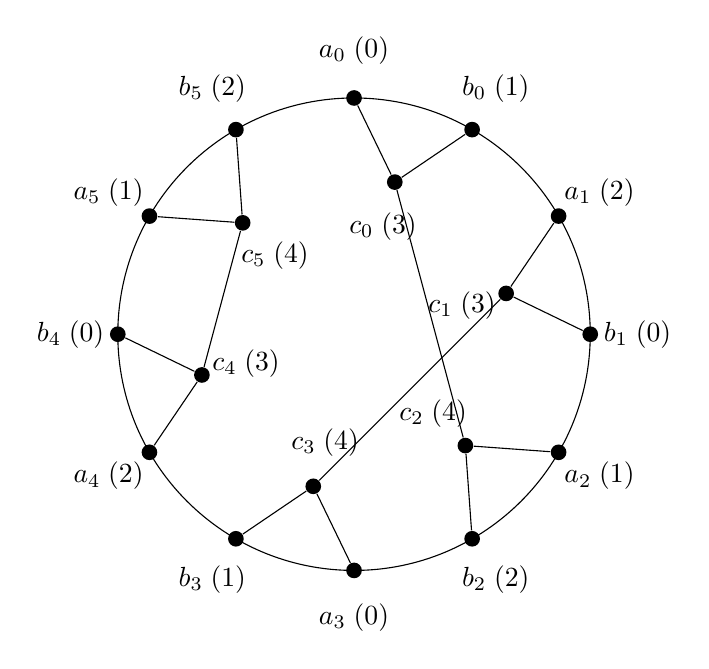
\begin{tikzpicture}[scale=1, transform shape,
    vertex/.style={circle, fill=black, inner sep=2pt}
]

% Círculo exterior
\draw (0,0) circle (3cm);

% Vértices a_i, b_i
\foreach \i/\name/\col in {
    0/$a_0$/0, 1/$b_0$/1, 2/$a_1$/2, 3/$b_1$/0,
    4/$a_2$/1, 5/$b_2$/2, 6/$a_3$/0, 7/$b_3$/1,
    8/$a_4$/2, 9/$b_4$/0, 10/$a_5$/1, 11/$b_5$/2}
{
    \node[vertex] (v\i) at ({90-30*\i}:3) {};
    \node [shift=({90-30*\i}:0.6)] at (v\i) {\name\;(\col)};
}

% Vértices c_i
\foreach \i/\name/\col in {
    0/$c_0$/3, 1/$c_1$/3, 2/$c_2$/4,
    3/$c_3$/4, 4/$c_4$/3, 5/$c_5$/4}
{
    \node[vertex] (c\i) at ({75-60*\i}:2) {};
    \node [shift=({75-60*\i}:-0.58)] at (c\i) {\name\;(\col)};
}

% Aristas a_i-c_i y b_i-c_i
\foreach \i in {0,...,5}
{
    \pgfmathtruncatemacro{\a}{2*\i}
    \pgfmathtruncatemacro{\b}{2*\i+1}
    \draw (v\a)--(c\i)--(v\b);
}

% Aristas del matching M
\draw (c0)--(c2);
\draw (c1)--(c3);
\draw (c4)--(c5);

\end{tikzpicture}

    \caption{The case $2r\equiv0\pmod3$ in the proof of
    Theorem \ref{thm:ham-clawfree}. In this case $2r=12$.
    In parentheses after each vertex label is shown the color
    assigned to that vertex.}
    \label{fig:2requiv0mod3}
\end{figure}

Whenever $\chi_3(F)\leq5$, repeated applications of
Proposition~\ref{prop:chi3Gleqchi3F} yield $\chi_3(G)\leq5$.
We now construct a $3$-dynamic $5$-coloring of $F$, except for the
small configurations that will be handled separately using
Lemma~\ref{lem:small-diamond-insertions}.
Suppose first that $2r\equiv0\pmod3$. Precolor $D$ with a standard
coloring $\phi$. Since $2r$ is a multiple of $3$, this coloring is
well defined and proper on $D$. For every $i$ (indices taken modulo
$r$), the vertices $b_{i-1}$ and $b_i$ receive distinct colors, and
so do $a_i$ and $a_{i+1}$.
Since $C=\{c_0,\ldots,c_{r-1}\}$ induces the perfect matching $M$,
extend $\phi$ by assigning colors $3$ and $4$ to the two endpoints of
each edge of $M$. Then $a_i$ sees distinct colors on $b_{i-1}$ and
$b_i$, together with the color of $c_i$, and $b_i$ sees distinct
colors on $a_i$ and $a_{i+1}$, together with the color of $c_i$.
Moreover, $c_i$ sees the two distinct colors of $a_i$ and $b_i$ and
the color of its neighbor in $M$. Hence every vertex has three
neighbors of pairwise distinct colors, and $\phi$ is a $3$-dynamic
$5$-coloring of $F$ (Figure~\ref{fig:2requiv0mod3}).
We may therefore assume from now on that
$2r\not\equiv0\pmod3$.

Suppose that every edge of $M$ joins two consecutive vertices of $C$.
After relabeling if necessary, we may assume that
\[
M=\{c_{2i}c_{2i+1}:0\leq i<r/2\}.
\]
We first consider the case $2r\equiv1\pmod3$. Since $r$ is even, either
$r=2$ or $r\geq8$.
If $r=2$, then $F\cong C_3\square K_2$. Since
$\chi_3(C_3\square K_2)=6$, we may assume that at least one diamond occurs in $G$.
Let $F'$ be obtained from $F$ by retaining exactly one such diamond.
By Lemma~\ref{lem:small-diamond-insertions},
$\chi_3(F')\leq5$. Since $G$ is obtained from $F'$ by inserting the
remaining diamonds, repeated applications of
Proposition~\ref{prop:chi3Gleqchi3F} yield $\chi_3(G)\leq5$.

Hence, we may assume that $r\geq8$. We precolor
$
a_0b_0a_1b_1\ldots a_{r-3}b_{r-3}
$
with a standard coloring $\phi$. We then set
$
\phi(c_0)=\phi(c_{r-3})=\phi(c_{r-1})=3,
\qquad
\phi(c_{r-2})=0,
$
and
$
\phi(a_{r-2})=\phi(b_{r-1})=4,\qquad
\phi(b_{r-2})=1,\qquad
\phi(a_{r-1})=2.
$
We color the remaining vertices of $C$ with colors $3$ and $4$ so that
the endpoints of every edge of $M$ receive distinct colors.
A direct check shows that the resulting coloring is proper and that the
three neighbors of every vertex receive pairwise distinct colors.
Hence $\phi$ is a $3$-dynamic $5$-coloring of $F$
(Figure~\ref{fig:cubic-consecutive}a).

We now consider the case $2r\equiv2\pmod3$. Since $r$ is even,
$r\equiv4\pmod6$. We first assume that $r\geq10$.
We precolor
\[
a_0b_0a_1b_1\ldots a_{r-5}b_{r-5}
\]
with a standard coloring $\phi$. We then set
$
\phi(c_0)=\phi(c_{r-1})=\phi(b_{r-3})
=\phi(a_{r-4})=3,
$
$
\phi(a_{r-2})=\phi(b_{r-1})
=\phi(c_{r-4})=\phi(c_{r-5})=4,
$
$
\phi(c_{r-2})=\phi(c_{r-3})=0,
$ and
$
\phi(a_{r-1})=\phi(b_{r-4})=1,
\qquad
\phi(b_{r-2})=\phi(a_{r-3})=2.
$
We color the remaining vertices of $C$ with colors $3$ and $4$ so that
the endpoints of every edge of $M$ receive distinct colors.
A direct check shows that the resulting coloring is proper and that the
three neighbors of every vertex receive pairwise distinct colors.
Hence $\phi$ is a $3$-dynamic $5$-coloring of $F$
(Figure~\ref{fig:cubic-consecutive}b).
Finally, If $r=4$, then
$
M=\{c_0c_1,c_2c_3\},
$
and hence $F\cong X_{12}$. If no diamond occurs, then
$G\cong X_{12}$; if exactly one diamond occurs, then
$G\cong X_{16}^1$ or $G\cong X_{16}^2$. It can be verified that $\chi_3(G)=6$ for any such $G$. Hence, assume that at least two diamonds occur in $G$.
Let $F'$ be obtained from $X_{12}$ by retaining exactly two of these
diamonds. By Lemma~\ref{lem:small-diamond-insertions},
$\chi_3(F')\leq5$. Since $G$ is obtained from $F'$ by inserting the
remaining diamonds, repeated applications of
Proposition~\ref{prop:chi3Gleqchi3F} yield $\chi_3(G)\leq5$.


\begin{figure}[H]
    \centering

    \begin{subfigure}{0.48\textwidth}
        \centering
        % \tikzexternaldisable


\tikzsetnextfilename{fig-cubic-consecutive-1}
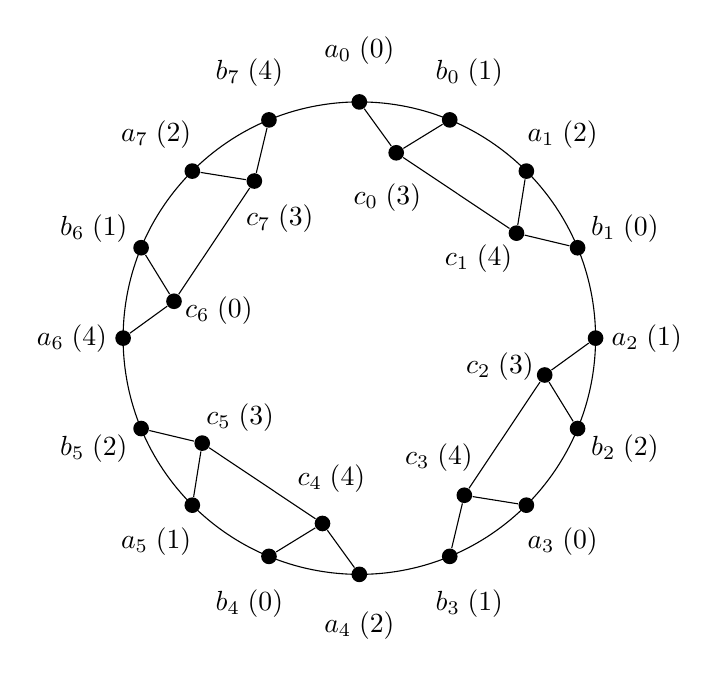
\begin{tikzpicture}[scale=1,
    vertex/.style={circle, fill=black, inner sep=2pt}
]

% Círculo exterior
\draw (0,0) circle (3cm);

% Vértices a_i, b_i
\foreach \i/\name/\col in {
    0/$a_0$/0, 1/$b_0$/1, 2/$a_1$/2, 3/$b_1$/0,
    4/$a_2$/1, 5/$b_2$/2, 6/$a_3$/0, 7/$b_3$/1,
    8/$a_4$/2, 9/$b_4$/0, 10/$a_5$/1, 11/$b_5$/2,
    12/$a_6$/4, 13/$b_6$/1, 14/$a_7$/2, 15/$b_7$/4}
{
    \node[vertex] (v\i) at ({90-22.5*\i}:3) {};
    \node [shift=({90-22.5*\i}:0.65)] at (v\i) {\name\;(\col)};
}

% Vértices c_i, centrados entre a_i y b_i
\foreach \i/\name/\col in {
    0/$c_0$/3, 1/$c_1$/4, 2/$c_2$/3,
    3/$c_3$/4, 4/$c_4$/4, 5/$c_5$/3,
    6/$c_6$/0, 7/$c_7$/3}
{
    \node[vertex] (c\i) at ({78.75-45*\i}:2.4) {};
    \node [shift=({78.75-45*\i}:-0.58)] at (c\i) {\name\;(\col)};
}

% Aristas a_i-c_i y b_i-c_i
\foreach \i in {0,...,7}
{
    \pgfmathtruncatemacro{\a}{2*\i}
    \pgfmathtruncatemacro{\b}{2*\i+1}
    \draw (v\a)--(c\i)--(v\b);
}

% Aristas del matching M
\draw (c0)--(c1);
\draw (c2)--(c3);
\draw (c4)--(c5);
\draw (c6)--(c7);

\end{tikzpicture}
        \caption{$ $}
    \end{subfigure}
    \hfill
    \begin{subfigure}{0.48\textwidth}
        \centering
        \tikzsetnextfilename{fig-cubic-consecutive-2}
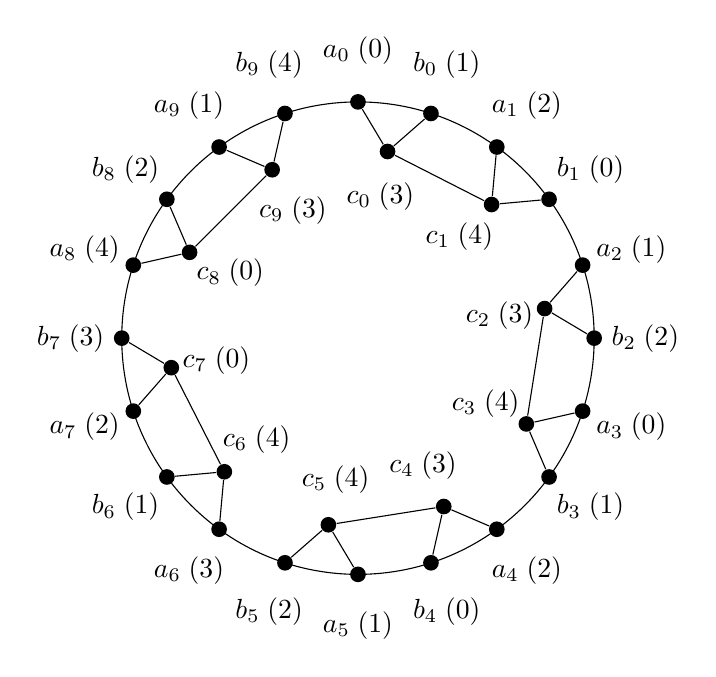
\begin{tikzpicture}[scale=1,
    vertex/.style={circle, fill=black, inner sep=2pt}
]

% Círculo exterior
\draw (0,0) circle (3cm);

% Vértices a_i, b_i
\foreach \i/\name/\col in {
    0/$a_0$/0,  1/$b_0$/1,
    2/$a_1$/2,  3/$b_1$/0,
    4/$a_2$/1,  5/$b_2$/2,
    6/$a_3$/0,  7/$b_3$/1,
    8/$a_4$/2,  9/$b_4$/0,
    10/$a_5$/1, 11/$b_5$/2,
    12/$a_6$/3, 13/$b_6$/1,
    14/$a_7$/2, 15/$b_7$/3,
    16/$a_8$/4, 17/$b_8$/2,
    18/$a_9$/1, 19/$b_9$/4}
{
    \node[vertex] (v\i) at ({90-18*\i}:3) {};
    \node [shift=({90-18*\i}:0.65)] at (v\i) {\name\;(\col)};
}

% Vértices c_i, centrados entre a_i y b_i
\foreach \i/\name/\col in {
    0/$c_0$/3, 1/$c_1$/4,
    2/$c_2$/3, 3/$c_3$/4,
    4/$c_4$/3, 5/$c_5$/4,
    6/$c_6$/4, 7/$c_7$/0,
    8/$c_8$/0, 9/$c_9$/3}
{
    \node[vertex] (c\i) at ({81-36*\i}:2.4) {};
    \node [shift=({81-36*\i}:-0.58)] at (c\i) {\name\;(\col)};
}

% Aristas a_i-c_i y b_i-c_i
\foreach \i in {0,...,9}
{
    \pgfmathtruncatemacro{\a}{2*\i}
    \pgfmathtruncatemacro{\b}{2*\i+1}
    \draw (v\a)--(c\i)--(v\b);
}

% Aristas del matching M
\draw (c0)--(c1);
\draw (c2)--(c3);
\draw (c4)--(c5);
\draw (c6)--(c7);
\draw (c8)--(c9);

\end{tikzpicture}
        %\caption{$2r\equiv2\pmod3$, $2r=20$.}
        \caption{$ $}
    \end{subfigure}

  \caption{The case in which every edge of $M$ joins two consecutive
vertices of $C$ in the proof of Theorem~\ref{thm:ham-clawfree}.
In parentheses after each vertex label is the color assigned to that
vertex. In (a), $2r\equiv1\pmod3$ and $2r=16$; in (b),
$2r\equiv2\pmod3$ and $2r=20$.}
    \label{fig:cubic-consecutive}
\end{figure}

We may therefore assume that $M$ contains an edge joining two
nonconsecutive vertices of $C$.
Among the edges $c_ic_k\in M$ joining nonconsecutive vertices of $C$,
choose one for which
$
\min\{|i-k|,\,r-|i-k|\}
$
is maximum. After relabeling the indices and, if necessary, reversing
their cyclic order, we may assume that this edge is $c_0c_j$, where
$
2\leq j\leq r/2.
$
Let
$
P=a_1b_1a_2b_2\ldots a_{j-1}b_{j-1}
$
and
$
Q=a_{j+1}b_{j+1}a_{j+2}b_{j+2}\ldots
a_{r-1}b_{r-1}.
$
Since
$
|V(P)|+|V(Q)|=2r-4
$
and $2r\not\equiv0\pmod3$, we have
$
|V(P)|+|V(Q)|\not\equiv2\pmod3.
$
Moreover, since $2\leq j\leq r-2$, both $P$ and $Q$ are nonempty.

Let $\overline{Q}$ denote the path $Q$ taken in the reverse order.
We precolor $P$ and $\overline{Q}$ with standard colorings $\phi$.
Thus, $\phi(a_1)=\phi(b_{r-1})=0$. We also set
$\phi(a_0)=\phi(c_1)=3$ and
$\phi(b_0)=\phi(c_{r-1})=4$.
We claim that $c_{j-1}$ and $c_{j+1}$ can be assigned distinct colors
from $\{3,4\}$ while preserving properness on the already colored edges
of $M$. If $j\geq3$, this follows directly from the fact that $M$ is a
matching. Suppose then that $j=2$. Since $c_1$ already has color $3$, we only
need to show that $c_3$ can receive color $4$. The only possible
obstruction is $c_3c_{r-1}\in M$. If $r\geq8$, this contradicts the
maximal choice of $c_0c_2$, since $c_3c_{r-1}$ has larger cyclic
distance. If $r=4$, then $c_3=c_{r-1}$ already has color $4$.

Thus, $c_{j-1}$ and $c_{j+1}$ can be assigned distinct colors from
$\{3,4\}$. By symmetry, we may assume that
$\phi(c_{j-1})=3$ and $\phi(c_{j+1})=4$. We then set
$\phi(a_j)=4$ and $\phi(b_j)=3$.
We color every remaining vertex of
$C\setminus\{c_0,c_j\}$ with colors $3$ and $4$ so that the endpoints
of every edge of $M$ other than $c_0c_j$ receive distinct colors.
At this point, every vertex outside $T_0\cup T_j$ satisfies the
$3$-dynamic condition. It remains to color $c_0$ and $c_j$.

First suppose that one of $|V(P)|$ and $|V(Q)|$ is congruent to $0$
modulo $3$. By symmetry, assume that $|V(P)|\equiv0\pmod3$.
Since $b_{j-1}$ is the last vertex of $P$, we have
$\phi(b_{j-1})=2$. Moreover, since
$|V(P)|+|V(Q)|\not\equiv2\pmod3$, we have
$|V(Q)|\not\equiv2\pmod3$. As $\overline{Q}$ is standard-colored,
it follows that $\phi(a_{j+1})\in\{0,2\}$.
We set $\phi(c_0)=2$ and $\phi(c_j)=1$. Since
$\phi(a_0)=3$, $\phi(b_0)=4$, and
$\phi(a_1)=\phi(b_{r-1})=0$, the coloring is proper and the
$3$-dynamic condition holds at the vertices of $T_0$.
Furthermore,
\[
\phi(b_{j-1})=2,\qquad
\phi(a_j)=4,\qquad
\phi(b_j)=3,\qquad
\phi(a_{j+1})\in\{0,2\}.
\]
Hence the coloring is proper and the $3$-dynamic condition also holds
at the vertices of $T_j$. Therefore, $\phi$ is a $3$-dynamic
$5$-coloring of $F$ (Figure~\ref{fig:cubic-notconsecutive}a).


\begin{figure}[H]
    \centering

    \begin{subfigure}{0.48\textwidth}
        \centering
        \tikzsetnextfilename{fig-cubic-P0mod3}
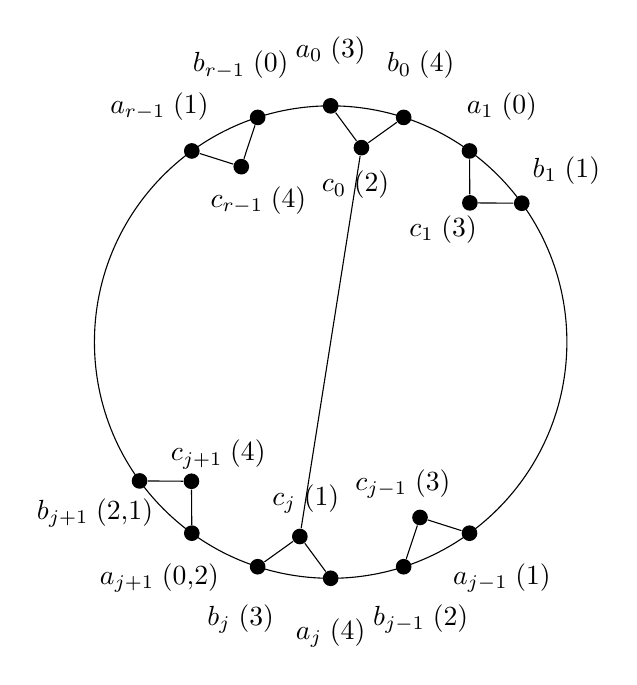
\begin{tikzpicture}[scale=1,
    vertex/.style={circle, fill=black, inner sep=2pt}
]

% Círculo exterior
\draw (0,0) circle (3cm);

% Vértices a_i, b_i
\foreach \i/\name/\col in {
    0/$a_0$/3,  1/$b_0$/4,
    2/$a_1$/0,  3/$b_1$/1,
    %4/$a_2$/1,  5/$b_2$/2,
    %6/$a_3$/0,  7/$b_3$/1,
    8/$a_{j-1}$/1,  9/$b_{j-1}$/2,
    10/$a_j$/4, 11/$b_j$/3,
    12/$a_{j+1}$/{0,2}, 13/$b_{j+1}$/{2,1},
    %14/$a_7$/2, 15/$b_7$/3,
    %16/$a_8$/4, 17/$b_8$/2,
    18/$a_{r-1}$/1, 19/$b_{r-1}$/0}
{
    \node[vertex] (v\i) at ({90-18*\i}:3) {};
    \node [shift=({90-18*\i}:0.7)] at (v\i) {\name\;(\col)};
}

% Vértices c_i, centrados entre a_i y b_i
\foreach \i/\name/\col in {
    0/$c_0$/2, 1/$c_1$/3,
    %2/$c_2$/3, 3/$c_3$/4,
    4/$c_{j-1}$/3, 5/$c_j$/1,
    6/$c_{j+1}$/4,
    %7/$c_7$/0, 8/$c_8$/0,
    9/$c_{r-1}$/4}
{
    \node[vertex] (c\i) at ({81-36*\i}:2.5) {};
    \node [shift=({81-36*\i}:-0.48)] at (c\i) {\name\;(\col)};
}

% Aristas a_i-c_i y b_i-c_i
% \foreach \i in {0,1,2,6,7,8}
\foreach \i in {0,1,4,5,6,9}
{
    \pgfmathtruncatemacro{\a}{2*\i}
    \pgfmathtruncatemacro{\b}{2*\i+1}
    \draw (v\a)--(c\i)--(v\b);
}

% Aristas del matching M
\draw (c0)--(c5);
%\draw (c2)--(c3);
%\draw (c4)--(c5);
%\draw (c6)--(c7);
%\draw (c8)--(c9);

\end{tikzpicture}
        \caption{$ $}
        \label{fig:2requiv1mod3}
    \end{subfigure}
    \hfill
    \begin{subfigure}{0.48\textwidth}
        \centering
        \tikzsetnextfilename{fig-cubic-P2mod3}
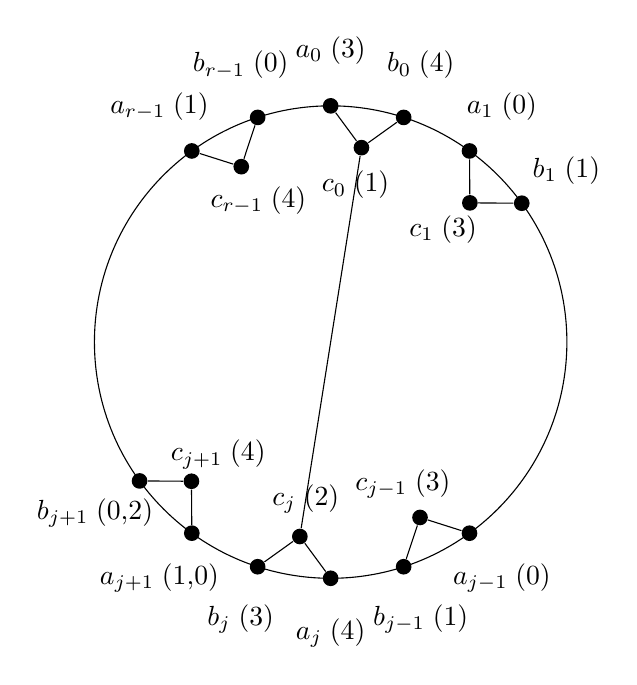
\begin{tikzpicture}[scale=1, 
    vertex/.style={circle, fill=black, inner sep=2pt}
]

% Círculo exterior
\draw (0,0) circle (3cm);

% Vértices a_i, b_i
\foreach \i/\name/\col in {
    0/$a_0$/3,  1/$b_0$/4,
    2/$a_1$/0,  3/$b_1$/1,
    %4/$a_2$/1,  5/$b_2$/2,
    %6/$a_3$/0,  7/$b_3$/1,
    8/$a_{j-1}$/0,  9/$b_{j-1}$/1,
    10/$a_j$/4, 11/$b_j$/3,
    12/$a_{j+1}$/{1,0}, 13/$b_{j+1}$/{0,2},
    %14/$a_7$/2, 15/$b_7$/3,
    %16/$a_8$/4, 17/$b_8$/2,
    18/$a_{r-1}$/1, 19/$b_{r-1}$/0}
{
    \node[vertex] (v\i) at ({90-18*\i}:3) {};
    \node [shift=({90-18*\i}:0.7)] at (v\i) {\name\;(\col)};
}

% Vértices c_i, centrados entre a_i y b_i
\foreach \i/\name/\col in {
    0/$c_0$/1, 1/$c_1$/3,
    %2/$c_2$/3, 3/$c_3$/4,
    4/$c_{j-1}$/3, 5/$c_j$/2,
    6/$c_{j+1}$/4,
    %7/$c_7$/0, 8/$c_8$/0,
    9/$c_{r-1}$/4}
{
    % \node[vertex] (c\i) at ({81-36*\i}:2.2) {};
    \node[vertex] (c\i) at ({81-36*\i}:2.5) {};
    \node [shift=({81-36*\i}:-0.48)] at (c\i) {\name\;(\col)};
}

% Aristas a_i-c_i y b_i-c_i
\foreach \i in {0,1,4,5,6,9}
% \foreach \i in {0,1,2,6,7,8}
{
    \pgfmathtruncatemacro{\a}{2*\i}
    \pgfmathtruncatemacro{\b}{2*\i+1}
    \draw (v\a)--(c\i)--(v\b);
}

% Aristas del matching M
\draw (c0)--(c5);
%\draw (c2)--(c3);
%\draw (c4)--(c5);
%\draw (c6)--(c7);
%\draw (c8)--(c9);

\end{tikzpicture}
        %\caption{$2r\equiv2\pmod3$, $2r=20$.}
        \caption{$ $}
        \label{fig:cubic-P0mod3}
    \end{subfigure}

    \caption{Situation in the proof
    of Theorem \ref{thm:ham-clawfree}. In this case, there exist an edge $c_0c_j$ with $j>0$. In parenthesis after each
    vertex label is shown the color assigned to such vertex. In $(a)$ we depict the case $|V(P)|\equiv 0\pmod3$.
    In $(b)$ we depict the case $|V(P)|\equiv 2\pmod3$.}
    \label{fig:cubic-notconsecutive}
\end{figure}

We may therefore assume that neither $|V(P)|$ nor $|V(Q)|$ is
congruent to $0$ modulo $3$. Since
$|V(P)|+|V(Q)|\not\equiv2\pmod3$, at least one of them is congruent
to $2$ modulo $3$. By symmetry, assume that
$|V(P)|\equiv2\pmod3$.
Then $\phi(b_{j-1})=1$. Moreover, $|V(Q)|\not\equiv0\pmod3$, and,
since $\overline{Q}$ is standard-colored,
$\phi(a_{j+1})\in\{0,1\}$.
We set $\phi(c_0)=1$ and $\phi(c_j)=2$. Again, since
$\phi(a_0)=3$, $\phi(b_0)=4$, and
$\phi(a_1)=\phi(b_{r-1})=0$, the coloring is proper and the
$3$-dynamic condition holds at the vertices of $T_0$.
Moreover,
\[
\phi(b_{j-1})=1,\qquad
\phi(a_j)=4,\qquad
\phi(b_j)=3,\qquad
\phi(a_{j+1})\in\{0,1\}.
\]
Thus the coloring is proper and the $3$-dynamic condition also holds
at the vertices of $T_j$. Therefore, $\phi$ is a $3$-dynamic
$5$-coloring of $F$ (Figure~\ref{fig:cubic-notconsecutive}b).
\end{proof}